\documentclass[10pt]{article}
\usepackage{multicol}
\usepackage{geometry}
\usepackage{amssymb}
\usepackage{amsmath}
\usepackage{mathunicode}
\usepackage{graphicx}

\geometry{left=0.5in, top=0.5in, right=0.5in, bottom=0.5in}
\graphicspath{.}
\title{how to math}
\author{nptnl}
\date{May 28, 2023}

\begin{document}
\begin{multicols}{2}

\maketitle

\section{The exponential function}

The exponential function $\exp(x) = e^x$ is the foundation of the exponentiation operator and all trigonometric functions.

\subsection{Maclaurin polynomial optimization}

The exponential function $\exp(x)$ is defined with a very specific property, that it is its own derivative function. This means $\exp(x)$ is also its own second derivative, third, and is indeed equal to all orders of its own derivatives. Hence, its Maclaurin polynomial simply becomes:

\[
    e^x = \exp(x) = ∑_{n=0}^∞ \frac{x^n}{n!} = \frac{x^0}{0!} + \frac{x^1}{1!} + \frac{x^2}{2!} + \frac{x^3}{3!} ...
\]

To make for a simpler and faster $\exp(x)$ function, notice that each term is equal to the previous term, multiplied by $x$ and divided by the next $n$.

\begin{align*}
    1 · \frac{x}{1} &= x \\
    x · \frac{x}{2} &= \frac{x²}{2} \\
    \frac{x^2}{2} · \frac{x}{3} &= \frac{x³}{6} ... \\
\end{align*}

This means a `running' variable can be used along with a `total' variable to more easily create each term in a sequence, adding to `total' each time.

\subsection{Range-fixing}

This Maclaurin polynomial will only accurately describe $\exp(x)$ for a small range of inputs, especially if we limit the terms used to a smaller number (Solvation uses seven terms). In order to `fix' our inputs, and only use numbers inside a small radius of 0 as inputs to the polynomial approximation, a variety of exponential properties can be used. Firstly, the real and imaginary parts of the input can be split like this, such that we only need to deal with the real and imaginary parts independently:

\[
    \exp(a+bi) = \exp(a) · \exp(bi), a∈ℝ, b∈ℝ
\]

The negative side of the Maclaurin series on $ℝ$ is considerably less accurate than the positive side, so negative values can be converted to positive ones like this:

\[
    \exp(a) = \frac{1}{\exp(-a)}
\]

Next, for real parts too large for a good approximation, the input can be divided by $e$ repeatedly until it falls within a small radius of 0.

\begin{align*}
    \exp(a) &= \exp(a · e^{-1}) + 1 \\
    &= \exp(a · e^{-2}) + 2 ... \\
    &= \exp(a · e^{-n}) + n \\
\end{align*}

Now that the real part is range-fixed, only the imaginary part remains. Becuase the function $e^{bi}$ repeats itself every $2π$, $b$ can be reduced to a value $-π < b ≤ π$ using the mod operator:

\[
    \exp(bi) = \exp(bi ± 2πi)
\]

Next, replacing the input $bi$ with $\frac{π}{2} - bi$ has the effect of negating only the real part of the output (again, because the output follows the unit circle).

\begin{align*}
    \exp(bi) &= -\Re(\exp(π - bi)) + \Im(\exp(π - bi)) \\
    \exp(bi) &= -\Re(\exp(-π - bi)) + \Im(\exp(-π - bi)) \\
\end{align*}

Applying this for $b$-values $>\frac{π}{2}$ or $<-\frac{π}{2}$ limits our range to $-\frac{π}{2} < b < \frac{π}{2}$. Now that both the real and imaginary parts have been range-fixed, the Maclaurin polynomial can be used to calculate $\exp(a+bi)$, provided that our code remembers the ways in which is must transform the output.

\section{The natural logarithm}

As the inverse of $\exp(x)$, $\ln(x)$ is also essential for the exponentiation operator and is the basis of inverse trigonometric functions.

\subsection{Taylor polynomial optimization}

The derivative of $\ln(x)$ is $x^{-1}$, and subsequent derivatives can be calculated with the power rule. These derivatives yield the Taylor series:

\[
    \ln(x) = ∑_{n=1}^∞ \frac{(x - 1)^n}{n}
\]

Taylor polynomial optimization works very similarly here, but instead of multiplying the denominator by the next $n$, it is simply incremented for each iteration. 16 terms of this polynomial are used in Solvation's approximation for $\ln(x)$, after more range-fixing is applied to the input.

\subsection{Range-fixing}

Because the real and imaginary parts of an input to $\exp(x)$ correspond to the magnitude and angle of the output, respectively, the magnitude and angle of an input to $\ln(x)$ correspond to the real and imaginary parts of the output. Hence, our input is first split into its magnitude and "unit vector" on the complex unit circle, like this:

\begin{align*}
    x &= |x| · u_x \\
    u_x &= \frac{x}{|x|}
\end{align*}

The magnitude $|x|$ is calculated using a square root, which will be covered later on. Once this magnitude is split from the new complex number, with magnitude 1, each will be subject to different range-fixing. To begin, the Taylor polynomial tends to be better-behaved for $|x|$ < 1, rather than slightly above 1. To move all inputs below 1, this property is used:

\[
    \ln(\frac{1}{|x|}) = -\ln(|x|)
\]

Next, we can use the inverse of a property used for $\exp(x)$, and multiply the input by $e$ until it is within a convergent range (remember, the Taylor series only converges very close to 1, and we've already got the magnitude $|x|$ somewhere between 0 and 1).

\begin{align*}
    \ln(|x|) &= \ln(|x| · e^1) - 1 \\
    &= \ln(|x| · e²) - 2 \\
    &= \ln(|x| · e³) - 3 ... \\
    &= \ln(|x| · e^n) - n \\
\end{align*}

This is repeated until the magnitude falls within a radius of accuracy for our polynomial approximation, using 16 terms. To range-fix the unit part, the unit circle is split into four sections, divided at $θ = \frac{π}{4}, \frac{3π}{4}, \frac{5π}{4}$, and $\frac{7π}{4}$. I'll call these sections $α, β, γ$, and $δ$.

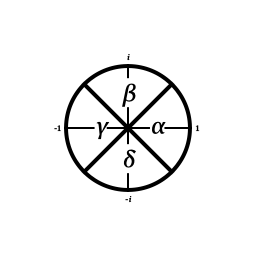
\includegraphics[scale=1.02]{ln-rf-diagram.png}

Inputs in region $α$ are already within an accurate range of the Taylor polynomial, the other three regions must be mapped into region $α$. To begin, assuming some complex number $u_x = a + bi$ of magnitude 1, inputs in region $γ$ can simply be negated, with $πi$ added to the output. Inputs in regions $β$ and $δ$ can be range-fixed using a rotation of $±\frac{π}{2}$:

\begin{align*}
    γ: \ln(a+bi) &= \ln((-1) · (-a-bi)) \\
    &= ln(-1) + ln(-a-bi) \\
    &= πi + ln(-a-bi) \\
    β: \ln(a+bi) &= \ln((-i) · (-b+ai)) \\
    &= \ln(-i) + ln(-b+ai) \\
    &= -\frac{π}{2}i + ln(-b+ai) \\
    δ: \ln(a+bi) &= \ln(i · (b-ai)) \\
    &= \ln(i) + ln(b-ai) \\
    &= \frac{π}{2}i + ln(b-ai) \\
\end{align*}

Once both the magnitude and unit circle number are range-fixed, the calculation reaches the optimized Taylor polynomial for $\ln(x)$, provided that the code remembers how it must transform the output.

\end{multicols}
\end{document}